\documentclass[12pt]{article}
\usepackage{amsmath}
\usepackage[margin=1 in]{geometry}
\usepackage{graphicx}
\usepackage{booktabs}
\usepackage{natbib}
\usepackage[colorlinks=true, citecolor=blue]{hyperref}
\usepackage{listings}
\usepackage{hyperref}

\title{Using Linear Regression to Examine the Correlation Between Access to Drinking Water and Life Expectancy}
\author{Julia Andronowitz\\
University of Connecticut\\Statistics Department}
\date{November 14, 2022}

\begin{document}

\maketitle

\begin{abstract}

\noindent
The aim of this paper is to assess the relationship between a population's access to potable drinking water and their average expected longevity. Data from the World Health Organization is filtered in Python before linear regression is performed. The paper then goes on to assess the correlation that exists as well as the assumptions for the model. Finally, improvements for the model and possible implications for the data are discussed along with overarching conclusions for the public health sector.

\end{abstract}

\section{Introduction}

\noindent
Living in the United States, we often take the necessity of safe drinking water for granted, but it is still a pressing issue in many parts of the world. Current research shows that unsafe water is responsible for millions of deaths \citep{ritchieroser2019water}. From the \textit{World Health Organization}, "Contaminated water and poor sanitation are linked to transmission of diseases such as cholera, diarrhoea, dysentery, hepatitis A, typhoid and polio" \citep{who2017water}. These diseases are largely preventable, and an increase in both access to and quality of safe drinking water can dramatically increase life expectancy \citep{angelakis2021quality}. Such a study could help emphasize the need for clean water worldwide, as it has numerous health benefits beyond longevity \citep{popkin2010waterhealth}. \\

\noindent
In the following sections, two data sets will be used to analyze how a population's access to clean drinking water can affect the average life expectancy. First, we will outline the background of the data. Then, we will go on to describe how to filter the data to what we are looking for and how linear regression is applied once the data is cleaned. Following this, we will discuss how the model was coded in Python and how various graphs were created. A summary of the model including the correlation we found and associated generated figures will be described. Finally, limitations of the study as well as future directions will be discussed.

\section{Data}

\noindent
The two data sets we will be using are from the World Health Organization and provided by Kaggle. The first is called Basic Drinking Water Services and contains information regarding basic drinking water services across various countries and in different years. There are 3455 rows with 4 columns: Location, Period, Indicator, and Tooltip. The indicator column is a text cell that says "Population using at least basic drinking-water services", and the Tooltip column gives the percentage of the population where the indicator is true. In this data set, we will be looking at the country, year, and percentage of population using at least basic drinking water services. \\
  
\noindent
The second data set is called Life Expectancy at Birth and contains information about life expectancy in various countries at the time of birth. It has 2197 rows and 5 columns: Location, Period, Indicator, Dim1, and Tooltip. In this data set, the indicator is the life expectancy at birth in years. The Dim1 column indicates which sex the life expectancy is referring to - male, female, or both sexes. For this data set, we will have to filter the rows to just contain those with a life expectancy for both sexes, as the other data set is not filtered by gender. We will be using the country and year columns to look at life expectancy.


\section{Methods}

\noindent
For the regression model, we start by loading the libraries that we will need. These include the Numpy, Pandas, and Bokeh libraries.

\begin{lstlisting}[language=Python]
import numpy as np
import pandas as pd
import seaborn as sns
from bokeh.plotting import figure
from bokeh.io import show, output_notebook
from bokeh.models import ColumnDataSource, HoverTool
from bokeh.layouts import gridplot
output_notebook()
\end{lstlisting}

\noindent
Next, we import the data:
\begin{lstlisting}[language=Python]
rawData1=pd.read_csv('archive/basicDrinkingWaterServices.csv')
rawData2=pd.read_csv('archive/lifeExpectancyAtBirth.csv')
\end{lstlisting}

\noindent
If we would like to see the data, use the command
\begin{lstlisting}[language=Python]
rawData1
\end{lstlisting}

\noindent
An output of the data is below:

\begin{center}
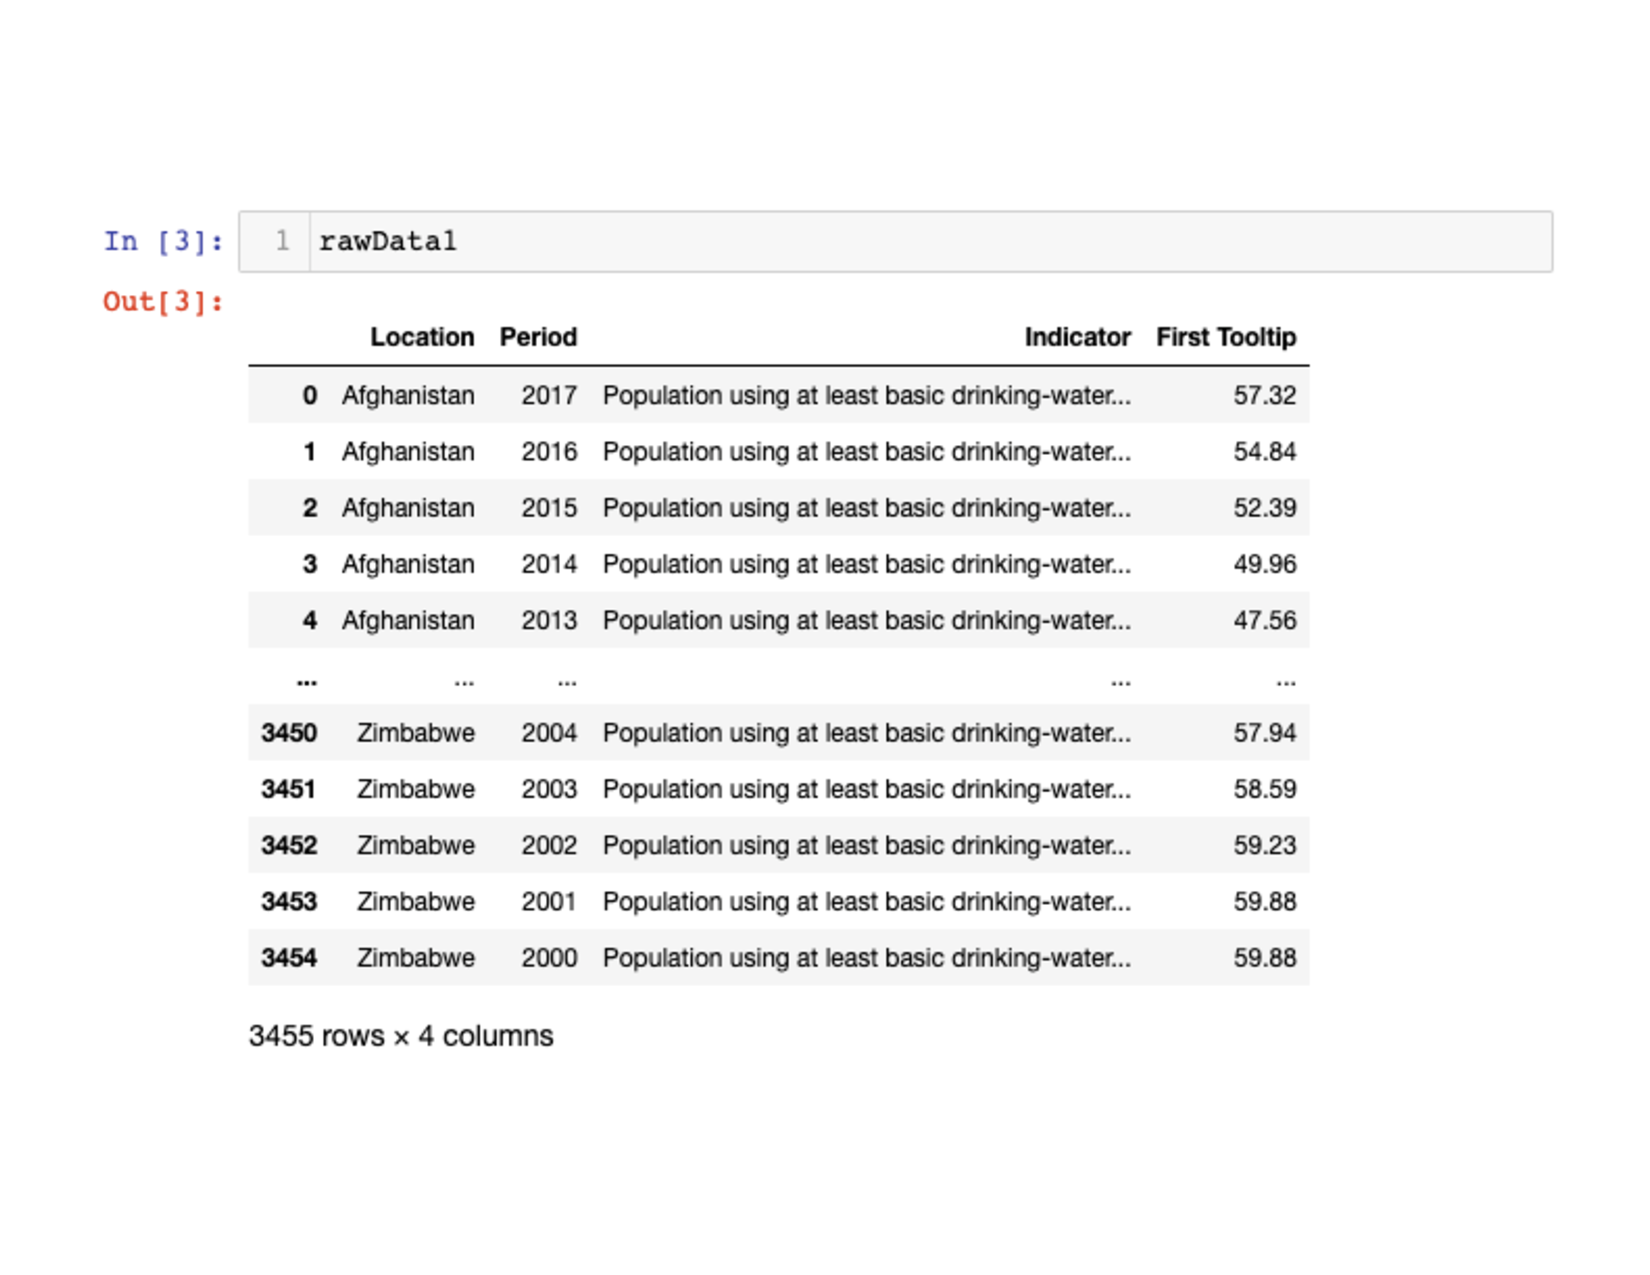
\includegraphics[width=5in]{Figures/data1.pdf}
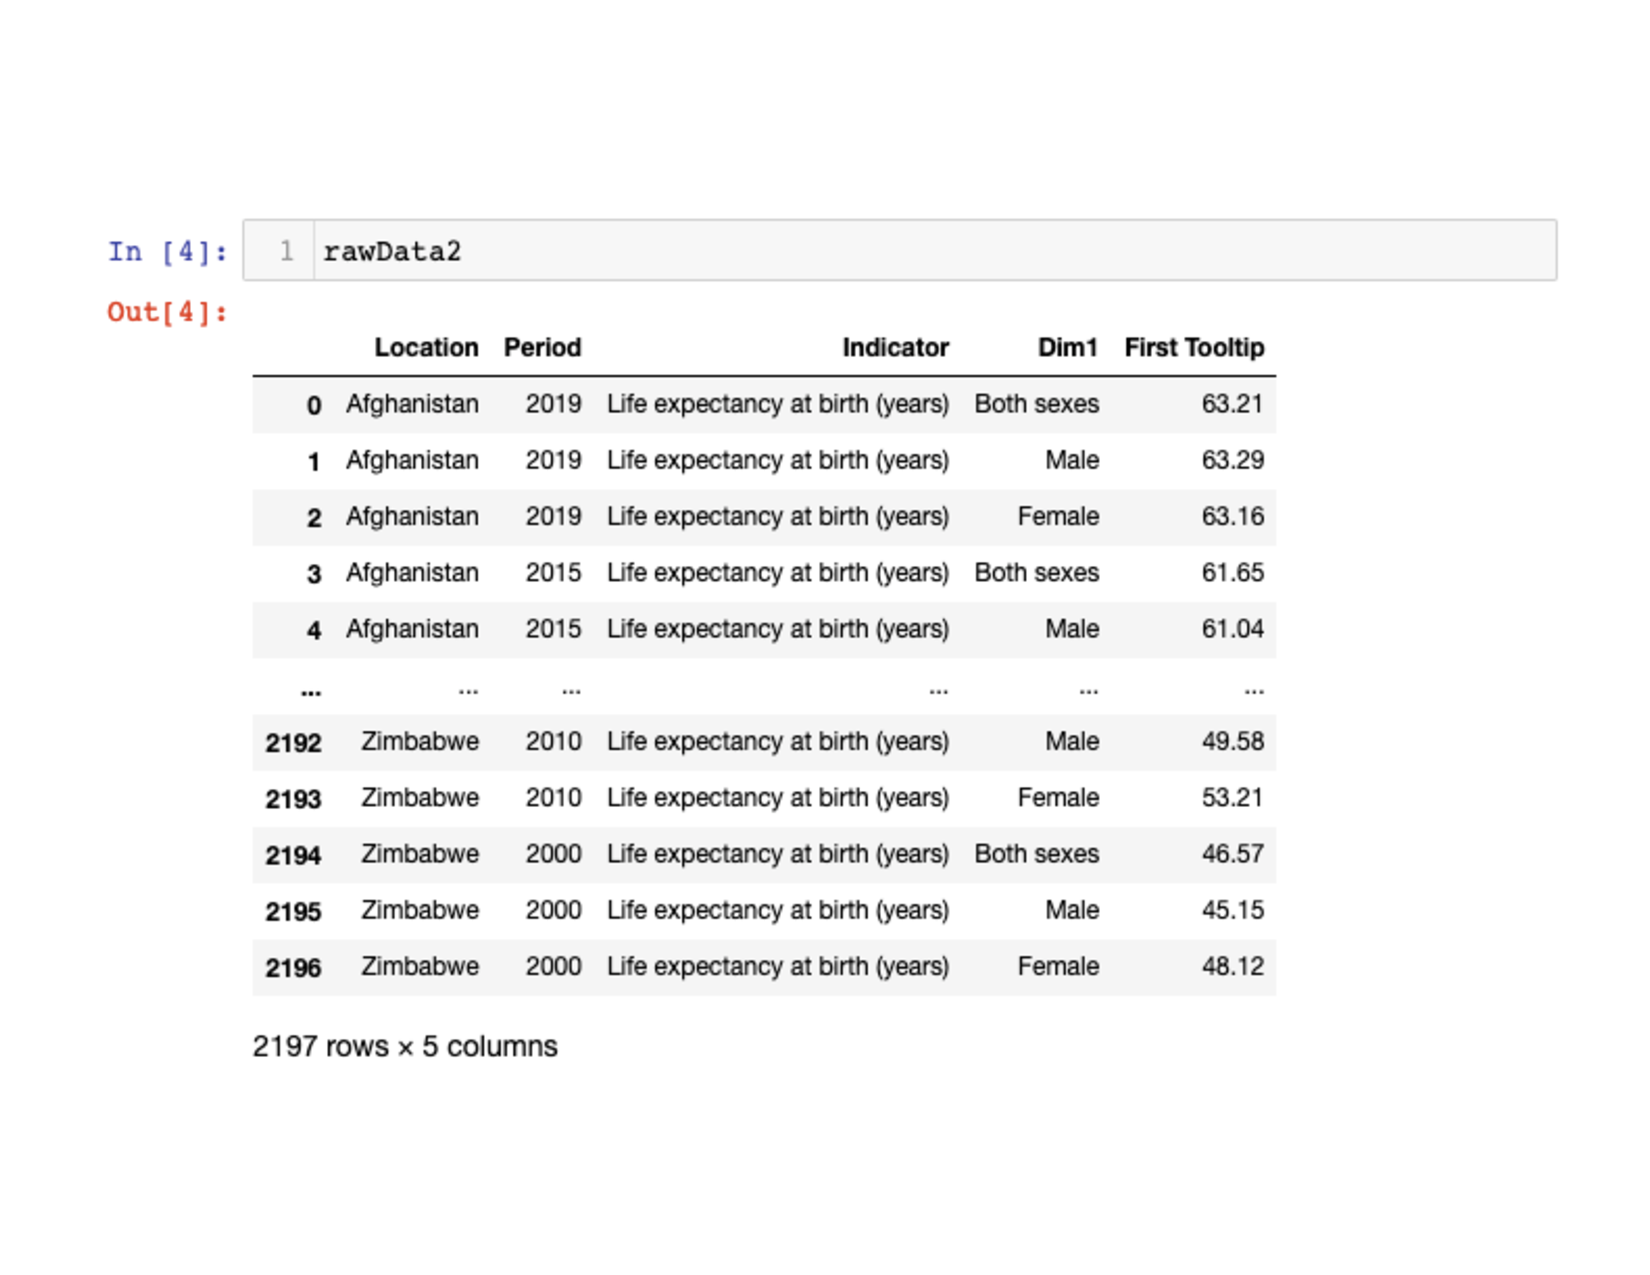
\includegraphics[width=5in]{Figures/data2.pdf}
\end{center}

\noindent
For the drinking water data, we take only the columns with the country, year, and the percentage of the population using at least basic drinking water services.
\begin{lstlisting}[language=Python]
rawData1=rawData1[["Location", "Period" , "First Tooltip"]]
\end{lstlisting}

\noindent
We do the same for the life expectancy data, only taking the columns with the country, year, sex, and average life expectancy at birth.
\begin{lstlisting}[language=Python]
rawData2=rawData2[["Location", "Period", "Dim1", "First Tooltip"]]
\end{lstlisting}

\noindent
Next, we want to convert our pandas dataframes into numpy arrays so that we can use the appropriate mathematical functions.
\begin{lstlisting}[language=Python]
data1=np.array(rawData1)
data2=np.array(rawData2)
\end{lstlisting}

\noindent
We want to have as many constants as possible in our model. Since the data was collected starting in 2000, we must use the same years in both data sets. We will use the year 2015 as the benchmark. The data can then be filtered using a loop and appending the 2015 data to a new list.
\begin{lstlisting}[language=Python]
dw2015=[]
for x in data1:
    if x[1]==2015:
        dw2015.append(x)
\end{lstlisting}

\noindent
This must be done for both data sets. We now do it for the life expectancy data set. As previously mentioned in the "Data" section, we also want to use only the rows with both sexes.
\begin{lstlisting}[language=Python]
le2015=[]
for x in data2:
    if (x[1]==2015) and (x[2]=='Both sexes'):
        le2015.append(x)
\end{lstlisting}

\noindent
These lists will also be converted into numpy arrays.
\begin{lstlisting}[language=Python]
DW2015=np.array(dw2015)
lifeExpectancy2015=np.array(le2015)
\end{lstlisting}

\noindent
Now, we see the shapes of both these arrays are different. The drinking water array contains 193 rows and 3 columns while the life expectancy array contains 183 rows and 4 columns. This means that there are some countries that are not in both lists. So, we need to delete the data for countries that are only in one or the other. We do this by checking if the countries in the drinking water array are also in the life expectancy data. If both countries are in both data sets, we append them to our new drinking water list, which is what we will use going forward.
\begin{lstlisting}[language=Python]
drinkingWater2015=[]
for x in DW2015:
    if x[0] in lifeExpectancy2015:
        drinkingWater2015.append(x)
drinkingWater2015=np.array(drinkingWater2015)
\end{lstlisting}

\noindent
Now, we can see the lists are the same length. If the lengths were still different, we could do the same process with the life expectancy list, i.e. making sure every country in the life expectancy list is also in the drinking water list and removing elements that are not. Next, we want to assign $x$ to the percentages of people with access to basic drinking water services and $y$ to the life expectancies in 2015.
\begin{lstlisting}[language=Python]
x2015=drinkingWater2015[:,2]
x2015=x2015.astype('float64')
y2015=lifeExpectancy2015[:,3]
y2015=y2015.astype('float64')
\end{lstlisting}

\noindent
Now that we have standardized data across the board, we can plot the life expectancy and basic drinking water.

\begin{center}
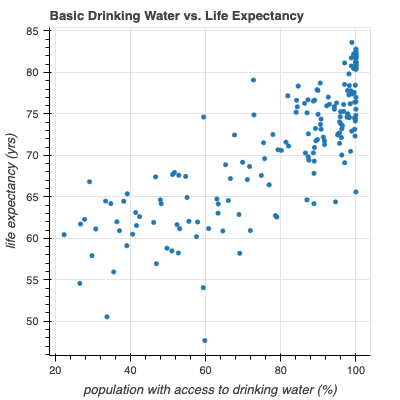
\includegraphics[width=6in]{Figures/figure1.png}\\
\end{center}

\begin{center}
    \textit{Figure 1.}
\end{center}

\noindent
Now we create our data matrix $x$, which is the $x$ array transformed into a column vector and appended to a column of ones.
\begin{lstlisting}[language=Python]
x2015=x2015.reshape(-1,1)
X2015=np.concatenate([x2015,np.ones(shape=(x2015.shape[0],1))],axis=1)
\end{lstlisting}

\noindent
Since this is now a column vector, we also want to transform $y$ into a column vector.
\begin{lstlisting}[language=Python]
Y2015=y2015.reshape(-1,1)
\end{lstlisting}

\noindent
Now, we can compute the least squares line and the matrix $M$ that will give us the slope and the $y$-intercept for the line of best fit.
\begin{lstlisting}[language=Python]
D2015=X2015.transpose()@X2015
np.linalg.inv(D2015)
M2015=(np.linalg.inv(D2015)@X2015.transpose())@Y2015
\end{lstlisting}

\noindent
The output is the array $[[0.27859093],[49.15736534]]$, which tells us the slope of the line is 0.279 and the intercept is 49.157. If we want to compare the actual values to predicted values, we use the following code:
\begin{lstlisting}[language=Python]
Yhat2015 = np.dot(np.dot(np.dot(X2015,np.linalg.inv(D2015)),
                                    X2015.transpose()),Y2015)
\end{lstlisting}

\noindent
A visual representation of the least squares line can be seen once executing
\begin{lstlisting}[language=Python]
f2015.line(x=x2015.ravel(),y=Yhat2015[:,0],color='black')
show(f2015)
\end{lstlisting}

\begin{center}
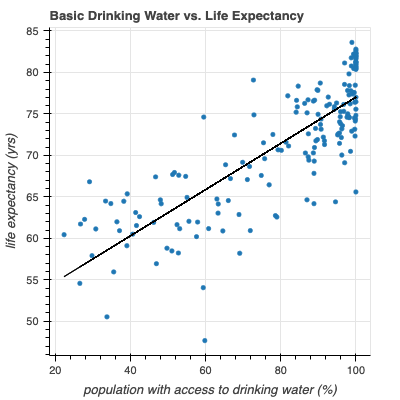
\includegraphics[width=6in]{Figures/figure2.png}\\
\end{center}

\begin{center}
    \textit{Figure 2.}
\end{center}

\section*{Assumptions}

\noindent
As seen in \textit{Figure 1}, we can assume a linear regression is appropriate for the model based on the data. There looks to be a linear correlation between the variables rather than a quadratic or other polynomial relationship. To see the R-Squared value of our linear regression, we can use the following code \citep{pythonr2}:
\begin{lstlisting}[language=Python]
corr_matrix = np.corrcoef(Y2015[:,0], Yhat2015[:,0])
corr = corr_matrix[0,1]
R_sq = corr**2
\end{lstlisting}
\noindent
We see the $R^2$ value is 0.66348. So, 66.348\% of the variability in the data is explained by the model. While this is on the lower end, our model is still supported. We would also like to check that the mean of the residuals is close to zero. This can be calculated with the following code.
\begin{lstlisting}[language=Python]
residuals=Yhat2015[:,0]-Y2015[:,0]
np.mean(residuals)
\end{lstlisting}
\noindent
We see the mean is -1.2813065726821479e-14 which is very close to zero. We also need to check for homosteadasticity among the residuals. To look at the residuals, the difference between the measured and predicted values, we can use the following function as detailed in \citet{teitelbaum2021linreg}.
\begin{lstlisting}[language=Python]
def comparison_plot(x,Y, Yhat):
    '''Plots Predicted vs True values for analysis of regression'''
    comparison_plot = 
        figure(title='Difference between Measured and Predicted Values')
    comparison_plot.xaxis.axis_label='x'
    comparison_plot.yaxis.axis_label='Yhat-Y'
    comparison_plot.scatter(x=x,y=Yhat-Y)
    comparison_plot.line(x=[x.min(),x.max()],y=[0,0])
    return comparison_plot
show(comparison_plot(x2015.ravel(),Y2015[:,0], Yhat2015[:,0]))
\end{lstlisting}

\begin{center}
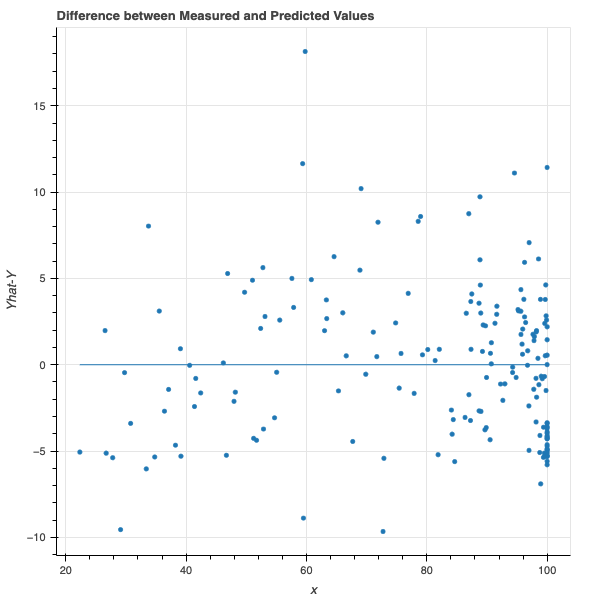
\includegraphics[width=4in]{Figures/figure3.png}\\
\end{center}

\begin{center}
    \textit{Figure 3.}
\end{center}

\newpage

\noindent
We see there are no patterns among the residuals, so this assumption is validated.

\vspace{15pt}

\noindent
Next, we would like to check for normality among the residuals. This can be achieved by plotting the distribution \citep{kaggleassumptions}.

\begin{lstlisting}
p = sns.displot(residuals,kde=True)
\end{lstlisting}

\begin{center}
    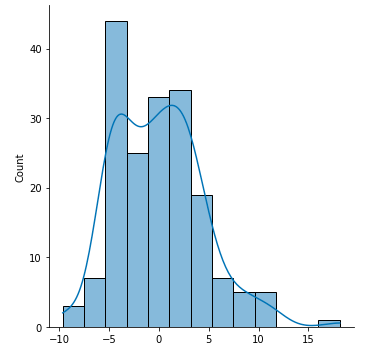
\includegraphics[width=6in]{Figures/figure4.png}\\
\end{center}

\begin{center}
\textit{Figure 4.}
\end{center}

\vspace{15pt}

\noindent
We see the graph is slightly bimodal but almost normally distributed as it is very hard to get perfectly normally distributed curves with real life.

\vspace{15pt}

\noindent
Finally, we look at possible outliers. The following code will calculate the studentized residuals and print values that are outside the normal range of (-3,3) \citep{statologyresiduals}.

\begin{lstlisting}
df = pd.DataFrame({'x': x2015[:,0],
                   'y': Y2015[:,0]})
model = ols('x ~ y', data=df).fit()
stud_res = model.outlier_test()

for x in stud_res['student_resid']:
    if x > 3 or x < -3:
        print(x)
\end{lstlisting}

\noindent
We see there is one outlier, with a studentized residual of -3.160. This outlier should be removed from the data set.

\section{Results}

\noindent
Most of the assumptions for linear regression were validated. The $R^2$ wasn't extremely high, but it still supported a positive correlation. Additionally, the mean of the residuals was extremely close to zero. Homeosteadasticity among the residuals was validated through a plot of the residuals. Since there were no patterns, this assumption is valid. Next, we checked the normality assumption. We observed a slightly bimodal distribution. Finally, our test for outliers resulted in one observation whose studentized residual was above 3. This outlier should be removed from the data set.

\vspace{15pt}

\noindent
From Figure 1, we see a general positive correlation between the two variables. This relationship illustrates that as the percentage of the population's access to safe drinking water increases, the average life expectancy also increases. Based on prior research, like that in \citet{angelakis2021quality} that suggests access to and quality of drinking water can increase an individual's life expectancy, this result was expected. Later on, we discovered the slope of the best fit line to be 0.279, and the $R^2$ value is 0.6638. This further supports our prediction that there would be a positive relationship between access to drinking water and life expectancy.

\vspace{15pt}

\noindent
From Figure 2 with the resulting best fit line, we see that some points are very close to the line while others are very far. Checking the plot of the residuals in Figure 3, we see there is a somewhat large variation between the predicted values and the measured values. Some of the values are extremely close to zero, meaning that there was little difference between the predicted value and the actual value. However, some of the values are closer to 10-15 away from zero, indicating a large difference between the predicted and measured values.

\section{Discussion}

\noindent
These results highlight the importance for access to clean drinking water, as we saw a positive correlation between access to safe water and life expectancy. We also saw some variation in the residuals, meaning that the model predicted a different outcome than the data points observed. The level of variation is a discrepancy between the predicted life expectancy of the model and the actual observed life expectancy from the data. This most likely has to do with the varying factors among different countries including other health factors such as air quality, sanitation, living conditions, and political stability. More conclusive research would have to be done to verify this. Possible methods such as multivariate regression and an analysis of covariance could be done. It is known that a person's health is affected by many factors, and a complete study to analyze just how much effect each factor has would be extensive. Though a study of this scale is improbable for this paper, such findings could revolutionize what public health organizations, governments, and citizens prioritize in relation to their health. This type of study has far-reaching effects and could not only improve a person's life expectancy but also their quality of life.

\vspace{15pt}

\noindent
This research paper focuses on investigating the effect of a population's access to clean drinking water on their life expectancy. We have found a positive correlation between the variables, which supports existing research that clean water is essential for the body to function. Insights in this field can further promote the basic right to safe water and highlight just how important water is in human health.


\newpage

\bibliography{References/References.bib}
\bibliographystyle{References/chicago.bst}

\end{document}